\section{Descripción del prototipo}
En este punto del trabajo terminal, este prototipo se encuentra en una fase aún experimental, sin embargo logra el 
cometido de simplificar el proceso de puesta en marcha.\\

Uno de los objetivos de la realización de este trabajo terminal es permitir al usuario empezar a hacer uso de Big Data de una manera sencilla y sin demasiadas complicaciones. Por lo que se comenzó el desarrollo de un instalador que simplifique el proceso de puesta en marcha del ambiente de análisis de datos.\\

La manera en que el instalador simplifica el proceso de instalación es automatizando algunas tareas que de otra forma el usuario tendría que realizar una a una, existiendo así la posibilidad de que éste mismo cometa algún error u omita algún paso, y por lo tanto, el ambiente de análisis de datos no pueda ponerse en funcionamiento.\\

Podría decirse que la utilidad de este prototipo se refleja al comparar el número de pasos que se enuncian en el manual de instalación de \emph{Luminus}, contra el número de pasos que se siguen al utilizar el instalador.\\

\section{Construcción y funcionamiento del prototipo}
Este prorotipo será ejecutado solamente desde la máquina queque sea el nodo maestro de la red distribuida. Deberá ser ejecutado. Al iniciar la ejecución del instalador, éste preguntará al usuario por la IP del nodo maestro. Luego preguntará por las IPs de los nodos que conformarán la red distribuida. Cada que el usuario introduzca una IP, el prototipo hará un ping para comprobar si hay conexión con el nodo cuya IP se desea agregar a la red distribuida. Si hay respuesta por parte del nodo en cuestión, se procede a almacenar ese dato en un archivo y se le pregunta al usuario si desea agregar otro nodo. Si su respuesta es afirmativa, este proceso se repite. 

\begin{figure}[H]
	\hypertarget{fig:hostnoencontrado}{\hspace{1pt}}
	\begin{center}	
		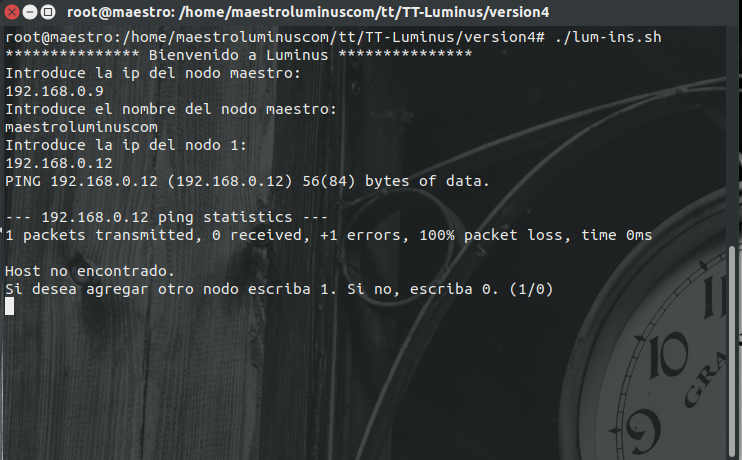
\includegraphics[width=.7\textwidth]{capitulo5/images/hostnoencontrado.png}
		\caption{El usuario introdujo la IP de un host no encontrado.}
	\end{center}
\end{figure}

\begin{figure}[H]
	\hypertarget{fig:hostencontrado}{\hspace{1pt}}
	\begin{center}	
		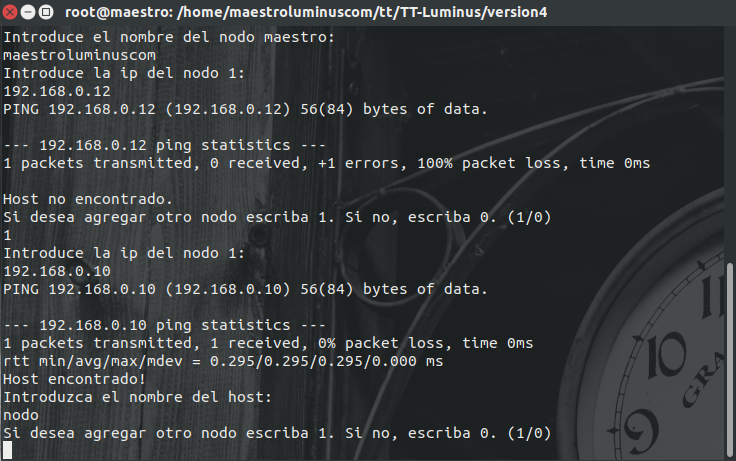
\includegraphics[width=.7\textwidth]{capitulo5/images/hostencontrado.png}
		\caption{El usuario introdujo la IP de un host encontrado.}
	\end{center}
\end{figure}

Posteriormente, cuando ya no se deseen agregar más nodos, el instalador ejecutará varios scripts de instalación en el nodo maestro, desde donde fue ejecutado.\\

\begin{figure}[H]
	\hypertarget{fig:instalacion}{\hspace{1pt}}
	\begin{center}	
		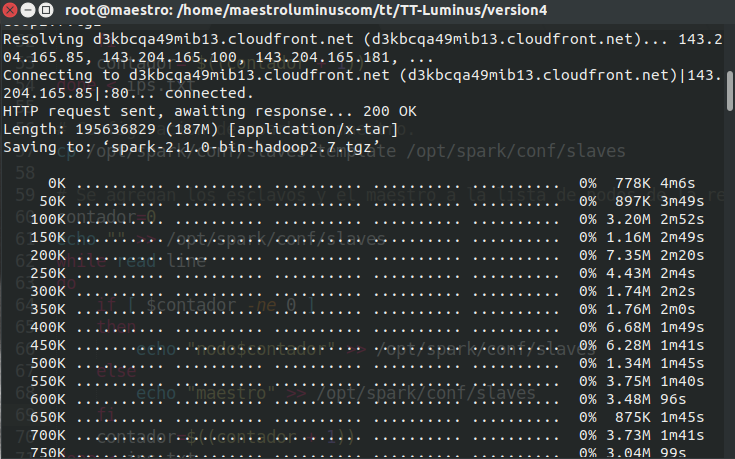
\includegraphics[width=.7\textwidth]{capitulo5/images/instalacion.png}
		\caption{Comienza el proceso de instalación.}
	\end{center}
\end{figure}

Estos scripts instalarán las tecnologías necesarias para que \emph{Luminus} pueda funcionar de manera adecuada. Estas tecnologías son las siguientes:\\

\begin{enumerate}
	\item Java.\\
	\item Scala.\\
	\item Spark.\\
\end{enumerate}

Después se procede a establecer conexiones SSH con los nodos de la red. Mediante SSH se ejecutan los mismos scripts que se ejecutaron en el nodo maestro pero de manera remota, es decir, sin la necesidad de tener almacenado el script en el nodo donde se va a iniciar la puesta en marcha del ambiente de análisis de datos.\\

Posteriormente se configura Spark en el nodo maestro, es decir, se asignan roles a los nodos de la red que introdujo el usuario al sistema en un principio.\\

Finalmente se realiza la instalación y configuración de Hadoop en el nodo maestro. Y por último en los demás nodos.

\newpage
\subsection{Diagrama de flujo}
\begin{figure}[H]
	\hypertarget{fig:diagramaFlujo}{\hspace{1pt}}
	\begin{center}
		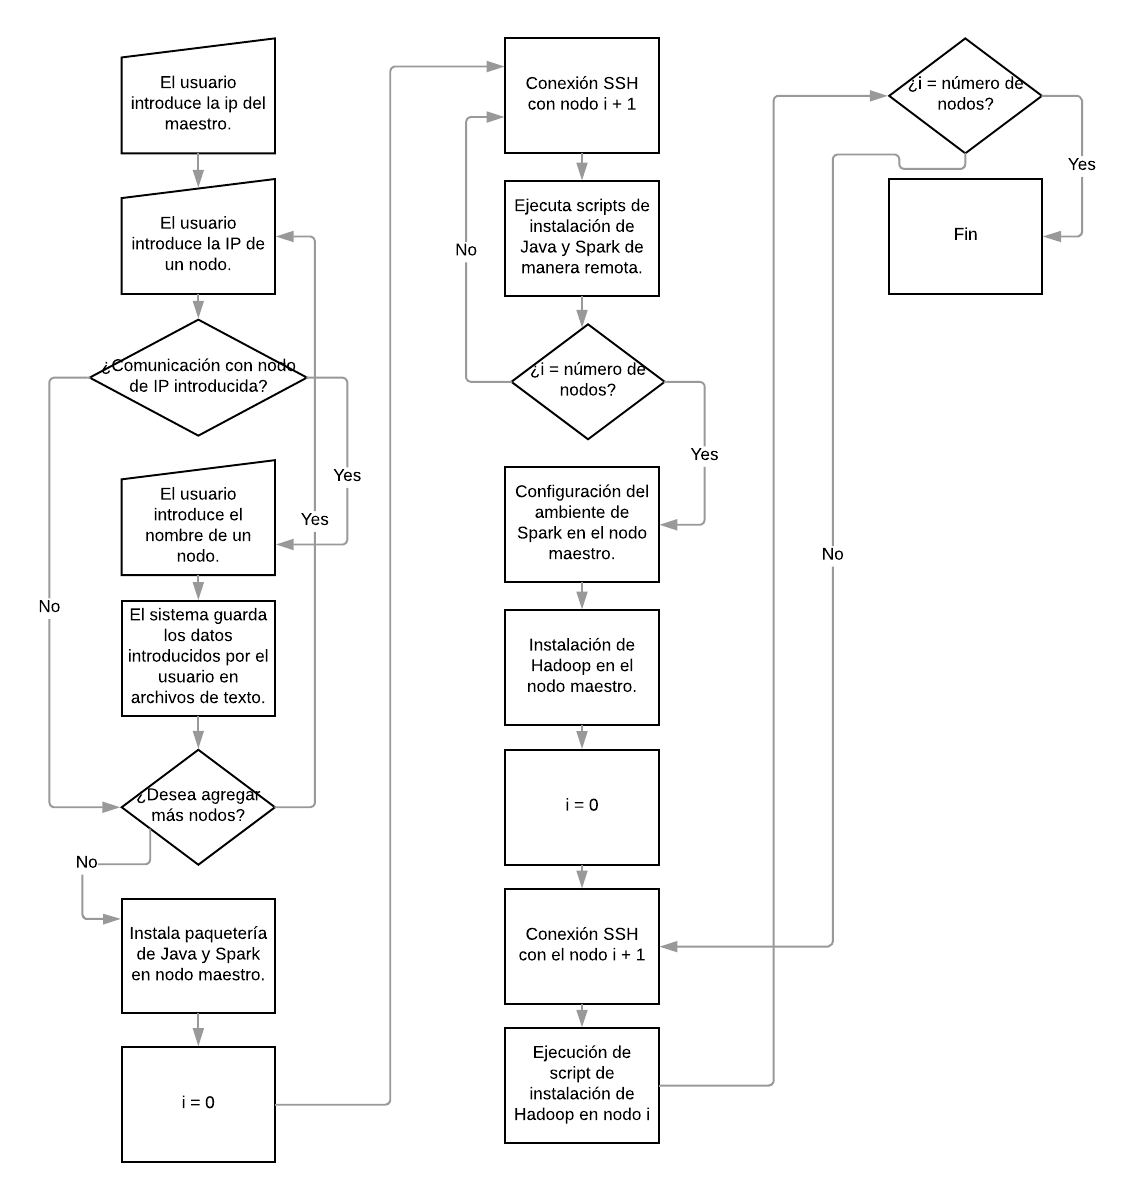
\includegraphics{capitulo5/images/diagramaFlujo.png}
		\caption{Diagrama de flujo de los pasos básicos que sigue el instalador.}
	\end{center}
\end{figure}

Este prorotipo se realizó por completo utilizando la tecnología Shell Script en Ubuntu 18.04.\\

\section{Alcances y trabajo a futuro}
Un instalador suele ser un sistema bastante complejo, ya que realiza las siguientes tareas:\\
\begin{itemize}
 	\item Instalación de software\\
 	\item Ejecuta comandos en el shell de la computadora\\
 	\item Verifica software que ya está instalado en la computadora y generalmente es capaz de cambiar la versión\\
\end{itemize}
Para la realización de este trabajo terminal, se pretende que durante el desarrollo del Trabajo Terminal 2, este prorotipo se vuelva más robusto de lo que es ahora, es decir:\\
\begin{itemize}
	\item Que sea capaz de reanudar el proceso de instalación cuando éste haya sido interrumpido. Ya sea por decisión del usuario o por un error en el proceso de instalación. El instalador, debe retomar el proceso a partir del punto en el que fue interrumpido.\\
	\item Que pueda agregar nodos a la red y remover nodos de la red.\\
	\item Que sea capaz actualizar las IPs de los nodos cuando exista algún cambio en ellas.\\
	\item Que pueda identificar si alguna de las tecnologías requeridas para la instalación de Luminus, ya existe en alguno de los nodos. De ser así, se validará la versión de la tecnología en cuestión. Si la versión es diferente a la que necesita Luminus, se pregunta al usuario si desea conservar su versión del software, o la versión necesaria para Luminus. Si la versión del software previamente instalada es la correcta, se notifica que Luminus no instaló esa tecnología.\\
\end{itemize}